The mathematical basis for the Finite Element Method begins in 1909
 with Ritz in which a continuous problem is replaced by 
a discrete problem with a finite number of degrees of freedom
 where the unknowns were approximated by the product between
 the constants to be determined and the base functions chosen
 in order to guarantee the accuracy of the result.
 This procedure is known as \textit{variational formulation}.
 Years later, Galerkin uses the Weighted Residual Method
 to determine the constants of the variational formulation
 where the same base functions were used in the weight functions.
 This procedure is known as \textit{Galerkin's formulation} and
 is widely used nowadays.

\medskip
During the 1940s, Courant (1943) \cite{courant1943} applied
 variational formulation to a domain discretized by triangular elements.
 In 1965, Zienkicwicz and Cheung \cite{zienkiewicz1965}
 show that the Weighted Residual Method has a good approximation
 of the solution and the Finite Element Method was formalized
 to solve several problems. The proposed mathematical approach
 is often used today.

\medskip
The Finite Element Method has become a very effective tool
 in the solution of several problems and it has been widely
 used in problems of the solids mechanics.
 In fluid mechanics, however, its use became possible only
 later due to the spurious oscillations that it can be seen
 when the convective term is superior to the diffusive term.
 Such oscillations are present not only in the Finite Element Method
 but were also observed in the Finite Difference Method by
 Spalding in 1972 \cite{spalding1972} where it is shown that
 the \textit{upwind} effect helped to reduce these oscillations.

\medskip
In 1976, Christie et al. \cite{christie1976} modify weight
 functions for asymmetric or quadratic functions to reduce
 spurious oscillations in one-dimensional diffusion-convection problems.
 Such modifications produced a \textit{upwind} effect on the solution.
 This procedure became known as \textit{Petrov Galerkin Formulation}.
 In the following year, Heinrich, Huyakorn and Zienkiewicz
 \cite{heinrich1977} generalize the scheme to a two-dimensional problem.
 The global matrices, however, became asymmetrical differently
 from those presented in the Galerkin scheme.

\medskip
In 1982, Brooks and Hughes \cite{brooks1982} proposed a
 new formulation that consists of modifying the weight functions
 so that the diffusion operator acts only in the flow direction.
 This procedure appears in order to eliminate the excess of
 diffusion perpendicular to the flow that
 the Petrov-Galerkin scheme presented in some cases.
 The formulation does not require the use of high-order
 weight functions and was efficient in eliminating perpendicular
 diffusion. The formulation received the name
 \textit{Streamline Upwind Petrov-Galerkin} (SUPG).


\medskip
In the same year, Pironneau \cite{pironneau1982} presented
 the Characteristic Curves Method applied to the
 Finite Element Method in solving the non-steady convection-diffusion
 and Navier-Stokes equations. Thereby, the author was able
 to derive conservative schemes of the type \textit{upwind}
 with first and second order accurate. As the matrices are symmetric,
 this scheme proved to be advantageous in solving linear
 systems compared to other \textit{upwind} schemes.
 Numerical implementation, however, requires numerical integration
 in the assembly of the vectors on the right side of the equation.
 This scheme initiates several works and is known later on as
 \textit {Characteristic Galerkin}.


\medskip
In 1984, Donea \cite{donea1984} presents an alternative for
 solving multidimensional and transient convection-diffusion
 problems. This alternative is known as the
 \textit{Taylor-Galerkin} scheme. The scheme consists of using
 the high-order terms of the Taylor expansion to reduce
 spurious oscillations. Unlike upwind schemes, in the
 Taylor-Galerkin scheme there is no need to use modified
 weight functions. The scheme is compared with the formulations
 of Galerkin and Petrov Galerkin and showed high precision and
 low numerical diffusion. Although the Taylor Galerkin and
 Characteristic Galerkin discretization procedures are distinct,
 the system of equations is identical for the convection-diffusion
 equation, where the unknowns is a scalar as mentioned by
 Lohner \cite{lohner1984}.

\medskip
Several researchers have analyzed the stability and convergencei
 of these schemes and even the implementation of more efficient
 schemes has emerged, such as the numerical simulation presented
 by Anjos et at. in 2006 \cite{anjos2006}, in which the
 \textit{semi-Lagrangean} scheme is implemented in the modeling
 of flows coupled to the transport of chemical species in
 a Finite Element approach. This scheme was widely used in
 meteorology and consists of calculating the material derivative
 along the characteristic trajectory. The discretization in time
 is done by first order backward differences while
 the discretization in space is performed according to
 the Galerkin scheme. The results showed that
 the semi-Lagrangian scheme is stable, showing no spurious
 oscillations and excessive numerical diffusion even
 for long time steps and high Reynolds and Schmidt numbers.
 Spurious oscillations in the Galerkin, SUPG and semi-Lagrangean
 schemes are compared by Silva (2011) \cite{silva2011} and
 theys are presented in \ref{spurious oscillations procedures}.

\begin{figure}[H]
     \begin{minipage}{.32\linewidth}
      \centering
      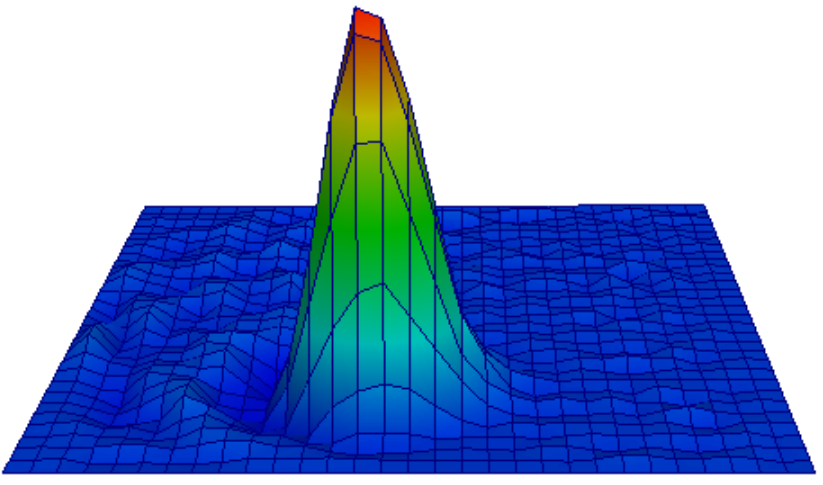
\includegraphics[scale=0.15]{./02_chaps/cap_review/figure/galerkin.png}\\
      (a)
     \end{minipage}%
     \begin{minipage}{.32\linewidth}
      \centering
      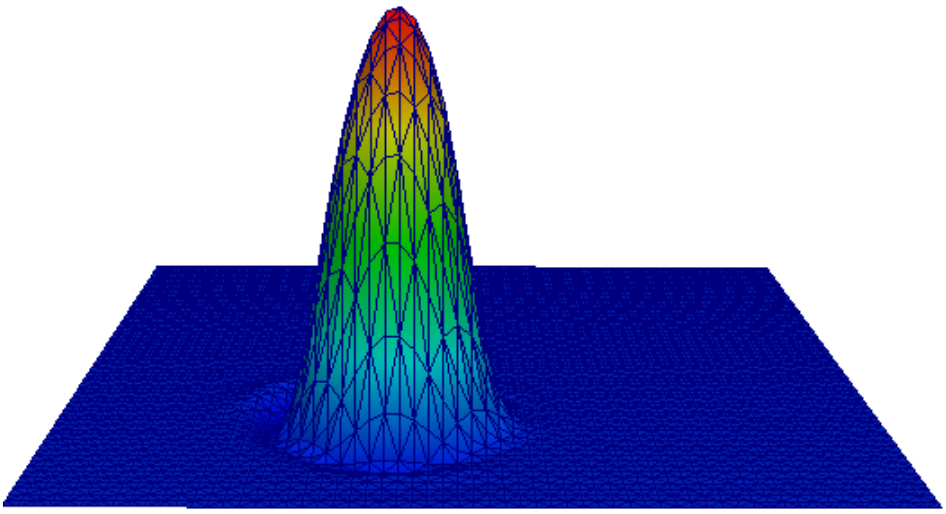
\includegraphics[scale=0.15]{./02_chaps/cap_review/figure/SUPG.png}\\
      (b)
     \end{minipage}%
     \begin{minipage}{.35\linewidth}
      \centering
      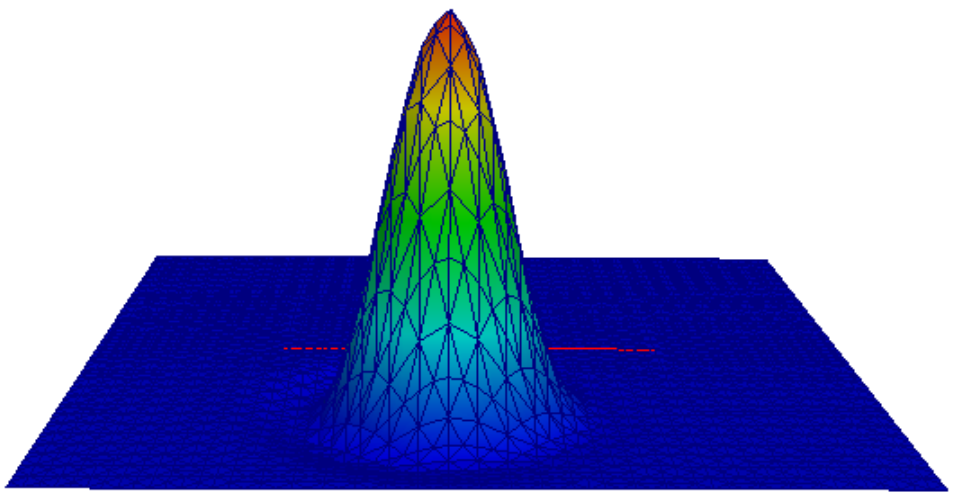
\includegraphics[scale=0.15]{./02_chaps/cap_review/figure/semilagrangian.png}\\
      (c)
     \end{minipage}%
     \medskip
     \caption{Comparison between spurious oscillations \cite{silva2011}:
              (a) Galerkin,
              (b) SUPG e 
              (c) semi-Lagrangian.}
     \label{procedimentos oscilacoes espurias}
\end{figure}



\medskip
The scheme choice to be used to reduce spurious oscillations
 is related to its advantages and disadvantages when compared
 to other schemes. In comparison to the Petrov-Galerkin and
 SUPG schemes, the Taylor-Galerkin, Characteristic and
 semi-Lagrangian schemes have the advantage of generating
 symmetric matrices facilitating computational implementation.
 Whereas, although the effectiveness of the semi-Lagrangian scheme
 is well known, it requires an efficient search algorithm for
 neighboring nodes to perform the interpolation.
 However, in Taylor-Galerkin and Characteristic Galerkin schemes,
 this need does not exist, so computational implementation becomes
 smooth. In addition, the system of linear equations generated by
 the Taylor-Galerkin scheme is similar to that generated by
 the Characteristic Galerkin scheme when the unknowns are scalar.
 Thus, the choice between these two schemes does not matter because 
 they produce similar results although the discretization process
 is different.

\medskip
All the schemes presented have satisfactory results and
they are well known in the literature.
 These schemes, therefore, made it possible to solve
 convective problems using the Finite Element Method.
 In this work, the semi-Lagragina scheme was chosen for
 the simulations.
